\documentclass[10pt]{beamer}
\usetheme[numbering=fraction]{metropolis}
\setbeamertemplate{frametitle continuation}{} % suppress "(i), (ii)..." on multi-part frames
\usepackage[T1]{fontenc}
\usepackage[utf8]{inputenc}
\usepackage{babel}
\usepackage{appendixnumberbeamer}
\usepackage{graphicx}
\usepackage{booktabs}
\usepackage{amsmath}
\usepackage{ragged2e}
\usepackage{bm}
\usepackage{csquotes}
\usepackage{multirow}
\usepackage[backend=biber,url=false,style=ieee]{biblatex}

\addbibresource{My Library.bib}

\renewcommand*{\bibfont}{\scriptsize}
\setbeamertemplate{bibliography item}[text]

\title{Towards Real-Time Ionospheric Scintillation Mitigation and Monitoring Using Radio Backpropagation}
\subtitle{Current Development and Goals}
\author{Rodrigo de Lima Florindo}
\institute{Aeronautics Institute of Technology}
\date{May 12, 2026}

\begin{document}

\maketitle

\begin{frame}{Overview}
    \tableofcontents
\end{frame}

\section{Introduction}

\begin{frame}{Introduction}
    \begin{itemize}
        \item With estimated single-frequency scintillation signals in hands, obtained from GNSS signal tracking, \parencite{breitschMitigationGlobalNavigation2023} have shown that it is possible to apply the \textbf{radio backpropagation method} for cycle-slips mitigation and to retrieve the original ionospheric refractive phase component associated with the scintillation-induced effects observed in GNSS signals.
        \item One of the main limitations of the radio backpropagation methodology presented in \parencite{breitschMitigationGlobalNavigation2023} is that it is restricted to offline data processing, \textit{i.e.}, it is necessary to accumulate many samples of the estimated scintillation signal.
        \item The goal of the current work is to extend the radio backpropagation approach to a real-time implementation. 
    \end{itemize}
\end{frame}

\begin{frame}{Introduction}
    \begin{itemize}
        \item The methodology shown in the following is intended to be performed in an online manner with scintillation signal estimation from carrier tracking outputs (scintillation intensity and phase must be available).
        \begin{itemize}
            \item Reliable detrended scintillation amplitude estimates are straightforward to be obtained from the prompt correlator outputs;
            \item We assume that the scintillation phase component (refractive + diffractive) can be retrieved in parallel with carrier tracking: Geometric, tropospheric, and TEC background models must be used to remove the most relevant phase features from carrier-phase estimates, leaving only the phase associated with the unmodeled scintillation effects.
        \end{itemize}
    \end{itemize}
\end{frame}


\section{The Split-Step Algorithm}

\begin{frame}{The Split-Step Algorithm}
    \begin{itemize}
        \item In the context of ionospheric scintillation models based on phase screen theory, the most used algorithm for approximating the paraxial differential wave equation that explains the ionosphere's refractive and the diffractive effects is known as the \textbf{split-step algorithm} \parencite[Section 2.2]{vasylyevModelingIonosphericScintillation2022}.
        \item This algorithm alternates between two sequential steps:
        \begin{enumerate}
            \item Refraction/interaction of a electromagnetic field with the ionosphere medium
            \item Propagation of the refracted field by filtering in the frequency domain using propagation kernel.
        \end{enumerate}
    \end{itemize}
\end{frame}

\begin{frame}{The Split-Step Algorithm}
    The split-step algorithm can be iteratively implemented as \parencite[Equations 9 and 10]{jiaoIonosphericScintillationSimulation2018}
    \begin{align}
        \label{eq:idft_phase_realization_simplified}
        \tilde{\psi}\left[0; n\right] &= \sum^{N-1}_{m=0}{\exp\left\{ j \overline{\phi}_{\mathrm{R}, l}\left[m\right] \right\} \exp\left\{ -2\pi j n m / N \right\}} \mathrm{,} \\
        \label{eq:post-prop_scint_field}
        \psi \left[\rho_{\mathrm{F}}; m\right] &= \frac{1}{N} \sum_{n=0}^{N-1} \tilde{\psi}\left[0; n\right]
        \exp \left\{ -j\left( n\Delta \mu \right)^2 /2 \right\}
        \exp \left\{ 2\pi j n m /N \right\} \mathrm{,}
    \end{align}
    where $\overline{\phi}_{\mathrm{R}, l}\left[m\right]$ is a phase realization sampled from a modeled power spectral density, $m$ is a discrete length in the eastward direction, and $n$ is its spatial frequency counterpart. $\rho_{\mathrm{F}} = \sqrt{x / k}$ denotes the Fresnel scale, where $k$ is the carrier's wavenumber, and $\Delta \mu = 2 \pi \Delta f \rho_{\mathrm{F}} / v_{\mathrm{eff}}$ is the normalized wavenumber resolution, with $v_{\mathrm{eff}}$ as the ionospheric piercing point effective scan velocity.
\end{frame}

\begin{frame}{The Split-Step Algorithm}
    Conversion from spatial to time domain can be achieved by substituing $\Delta \mu = 2 \pi \Delta f \rho_{\mathrm{F} / v_{\mathrm{eff}}}$ into, yielding
    \begin{align}
        \psi\left[ k \right] &= \frac{1}{N} \sum_{n=0}^{N-1} \tilde{\psi}\left[0; n\right]
        \exp \left\{ -j\left( 2\pi f \rho_{\mathrm{F}} / v_{\mathrm{eff}} \right)^2 /2 \right\}
        \exp \left\{ 2\pi j n m /N \right\} \mathrm{,}
    \end{align}
    where $k$ is the discrete time step and $f = f$ is its frequency counterpart. Note that the propagation operation is therefore fully described by this filtering operation of a phase-shifted field $\tilde{\psi}\left[0; n\right]$ through the filter
    \begin{align}
        H_{\mathcal{P}} \left[ f \right] = \exp \left\{ -j\left( 2\pi f \rho_{\mathrm{F}} / v_{\mathrm{eff}} \right)^2 /2 \right\}
    \end{align}
    whose group delay is given by
    \begin{align}
        \tau_{g} \left[ f \right] = -\frac{d \angle H_{\mathcal{P}} \left[ f \right]}{d \omega} \bigg \vert_{\omega = 2 \pi f} = 2 \pi f \left( \rho_{\mathrm{F}} / v_{\mathrm{eff}} \right)^2 \mathrm{,}
    \end{align}
\end{frame}

\begin{frame}{The Split-Step Algorithm}
    The propagation operator is an all-pass dispersive filter: it preserves the spectrum magnitude while imposing a linear group-delay profile, so higher temporal-frequency components experience larger delays and produce the observed diffractive interference pattern.

    As a single phase-screen is often used for modeling equatorial ionospheric scintillation, as it is done in the compact phase-screen-based scintillation model \parencite{rinoCompactMultifrequencyGNSS2018}, we consider only the case of a single phase screen in this work.
\end{frame}

\section{Radio Backpropagation}

\begin{frame}{Radio Backpropagation}
    Radio backpropagation consists in undoing the propagation step from the split-step algorithm by filtering a propagated signal with an estimate of the inverse propagation filter $\hat{H}_{\mathcal{P}}^{-1} \left( f \right) = \exp \left\{ j\left( 2\pi f \widehat{\rho_{\mathrm{F}} / v_{\mathrm{eff}}} \right)^2 /2 \right\}$, \textit{i.e.},
    \begin{align}
        \psi_{\mathrm{BP}} \left[ k \right] = {\mathrm{FFT}}^{-1} \left\{ \mathrm{FFT}\left\{ \psi \left[ k \right] \right\}\hat{H}_{\mathcal{P}}^{-1} \left( f \right) \right\} \mathrm{.}
    \end{align}
    In the case $\hat{H}_{\mathcal{P}} = H_{\mathcal{P}}$, it would be possible to fully retrieve the initating complex field at the ionospheric piercing point, without any diffractive effect. One benefit of applying this technique is that it does not need any knowledge on the statistics of the phase-screen realization. However, two issues become evident: a full batch of scintillation signal samples to apply the inverse of the estimated propagation kernel, and it is necessary to have an estimate $\widehat{\rho_{\mathrm{F}} / v_{\mathrm{eff}}}$.
\end{frame}

\section{Towards Real-Time Backpropagation}

\begin{frame}{Towards Real-Time Backpropagation}
    For now, assume that a reliable estimate of $\rho_{\mathrm{F}} / v_{\mathrm{eff}}$ is available and used to obtain the estimated inverse propagation filter $\hat{H}_{\mathcal{P}, M}^{-1}\left(f\right)$ evaluated over the $M$-point frequency support $f$. Instead of performing backpropagation in the full batch of samples, one may apply the estimated inverse propagation filter using a sliding window with latency $L$. Thus, a local backpropagated field can be obtained using
    \begin{align}
        \label{eq:sliding_bp}
        \psi_{\mathrm{BP}, L}^{\mathrm{sliding}}\left[k\right]
        &=
        \left[
        \mathrm{FFT}_{M}^{-1}
        \left\{
        \mathrm{FFT}_{M}
        \left\{
        w\left[r\right]\psi_{k,L}^{\mathrm{blk}}\left[r\right]
        \right\}
        \hat{H}_{\mathcal{P}, M}^{-1}\left(f\right)
        \right\}
        \right]_{r=M_{\mathrm{c}}}, \\
        \psi_{k,L}^{\mathrm{blk}}\left[r\right]
        &=
        \begin{cases}
            \psi\left[k+r-M_{\mathrm{c}}\right],
            & 0 \leq r \leq M_{\mathrm{c}} + L, \\
            \widehat{\psi}_{k,L}\left[ r \right],
            & M_{\mathrm{c}} + L < r \leq M-1,
        \end{cases}
        \quad
        M_{\mathrm{c}} = \left\lfloor M/2 \right\rfloor \mathrm{.}
    \end{align}
    where $\mathrm{FFT}_{M}$ and $\mathrm{FFT}^{-1}_{M}$ refer to an $M$-point FFT and inverse FFT, respectively, $w \left[ r \right]$ represents a windowing function, and $\widehat{\psi}_{k,L}\left[r\right]$ is a forecast for $\psi\left[k+r-M_{\mathrm{c}}\right]$ using samples available up to $k+L$.
\end{frame}

\begin{frame}{Towards Real-Time Backpropagation}
    We chose the sliding-window FFT as noncausal because the reliable output of each finite FFT block is the center sample. The inverse propagation filter has temporal spread, so estimating the backpropagated field at time $k$ requires signal context on both sides of $k$; otherwise, the estimate is dominated by block-edge artifacts.

    Note that this method is only feasible under the following conditions:
    \begin{enumerate}
        \item $M$ is sufficiently high, such that the sliding backpropagated field $\psi_{\mathrm{BP}, L}^{\mathrm{sliding}}\left[k\right]$ is sufficiently close to the backpropagated signal in batch $\psi_{BP} \left[ k \right]$;
        \item The unavailable future samples from $k+L+1$ to $k+M-M_{\mathrm{c}}-1$ can be predicted with sufficient accuracy. For $L=M-M_{\mathrm{c}}-1$, the method becomes full noncausal sliding window BP, and for $L = 0$, the backpropagation approach occurs in real time.
    \end{enumerate}
\end{frame}

\begin{frame}{Towards Real-Time Backpropagation}
    \centering
    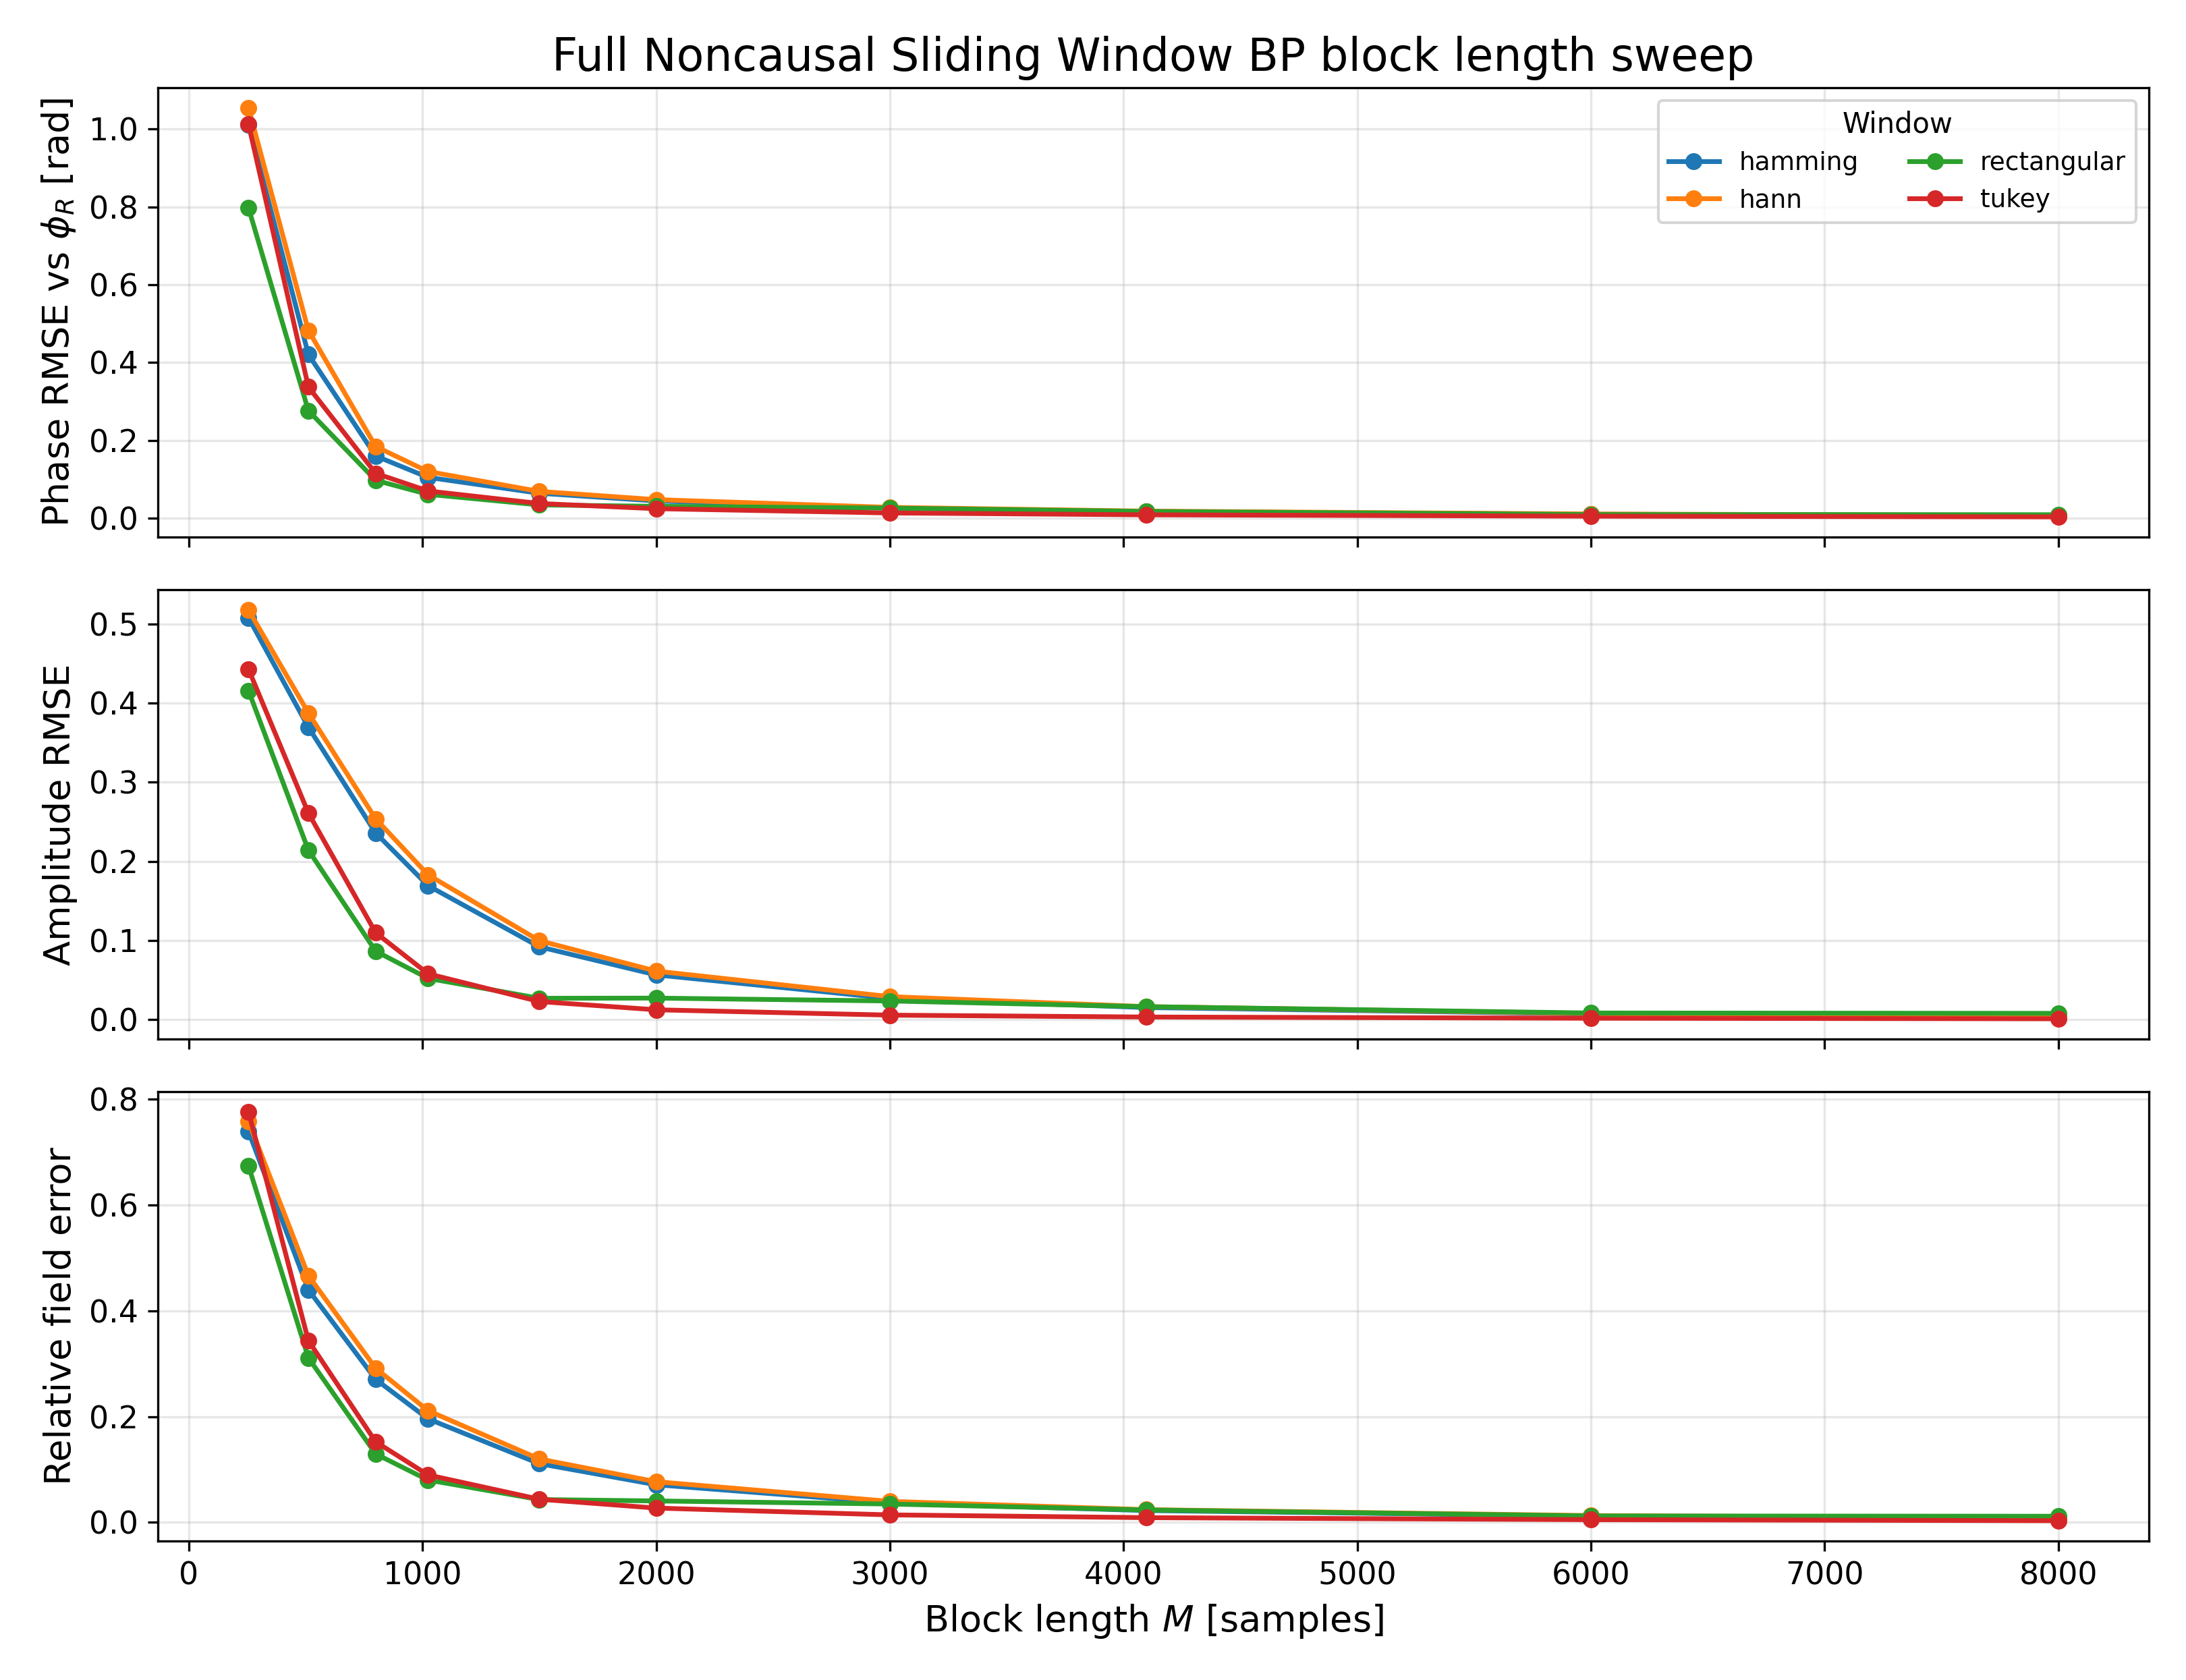
\includegraphics[width=0.85\linewidth]{../figures/sliding_window_bp_with_buffer_error_summary.png}
    \\\vspace{0.5em}
    \small Figure 1: Error metrics for full noncausal backpropagation using different windowing functions (using $L = M - M_c - 1$; without forecasting)
\end{frame}

\begin{frame}{Towards Real-Time Backpropagation}
    \centering
    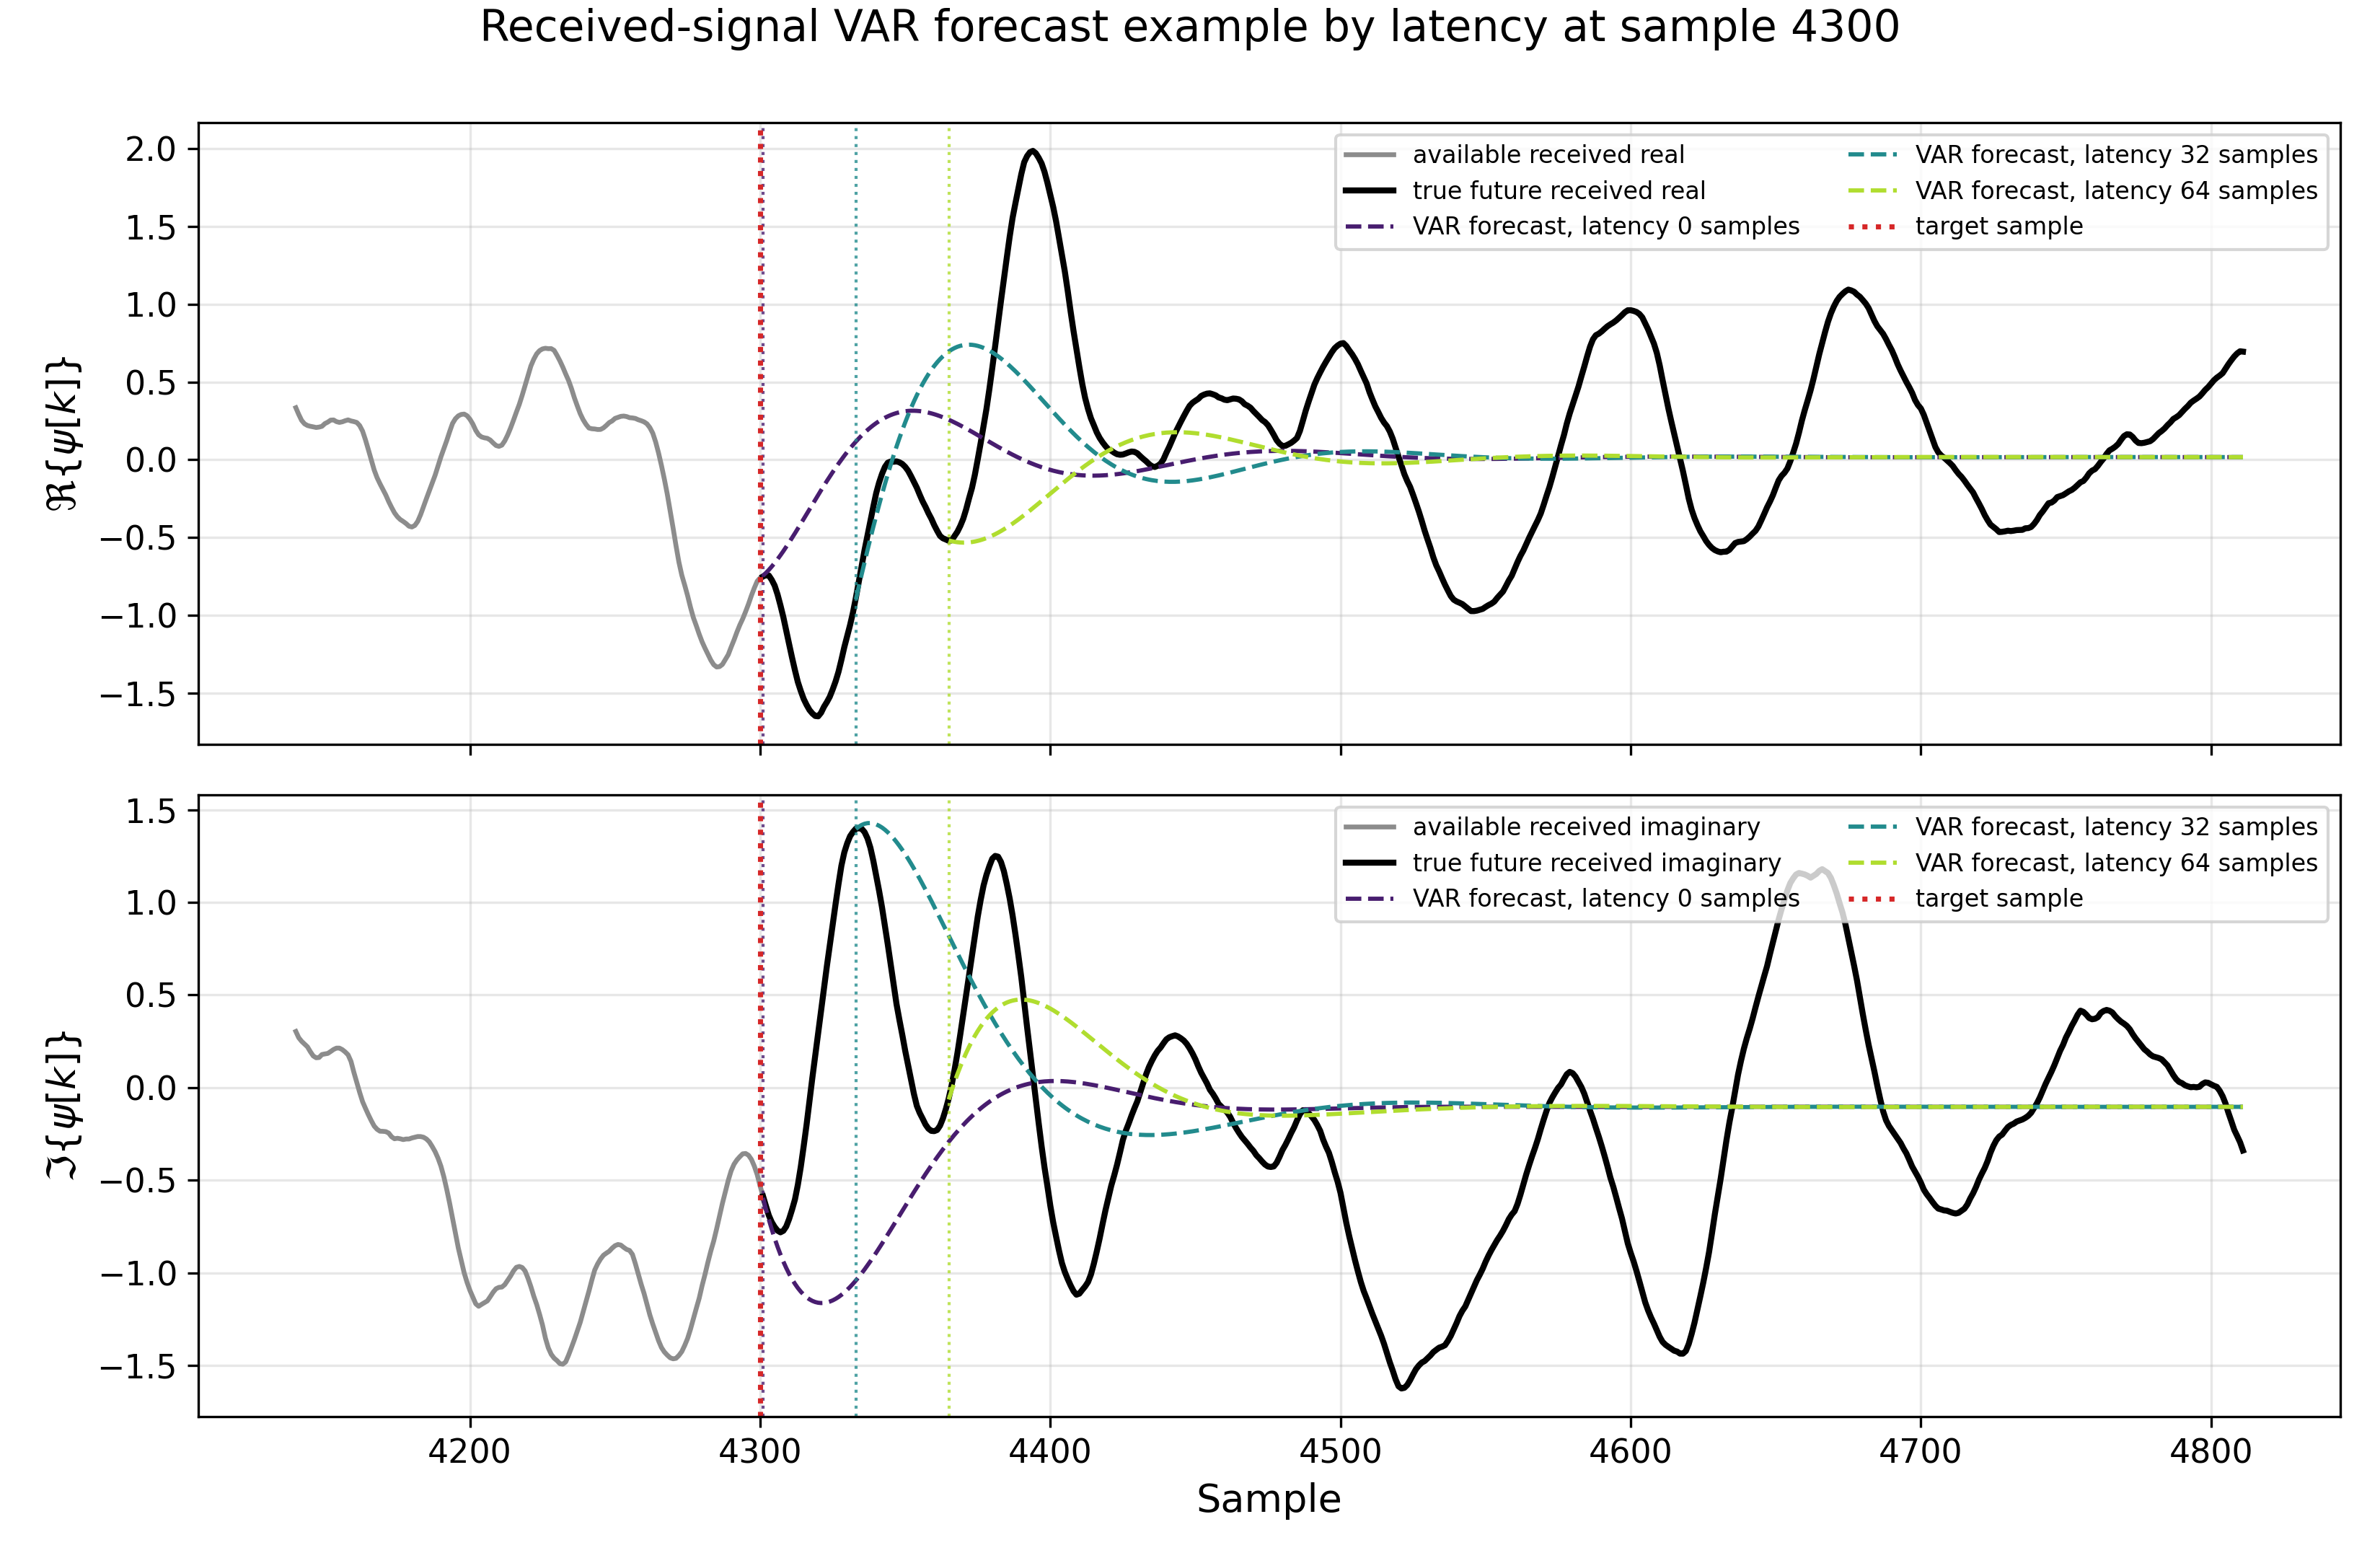
\includegraphics[width=0.9\linewidth]{../figures/real_imag_var_forecast_example_complex_parts.png}
    \\\vspace{0.5em}
    \small Figure 2: Example of forecasts provided by VAR models with different $L$. The VAR model with order 4 was employed for the real and imaginary parts of the estimated scintillation signal. The first 3500 samples were used to fit the model.
\end{frame}

\begin{frame}{Towards Real-Time Backpropagation}
    \centering
    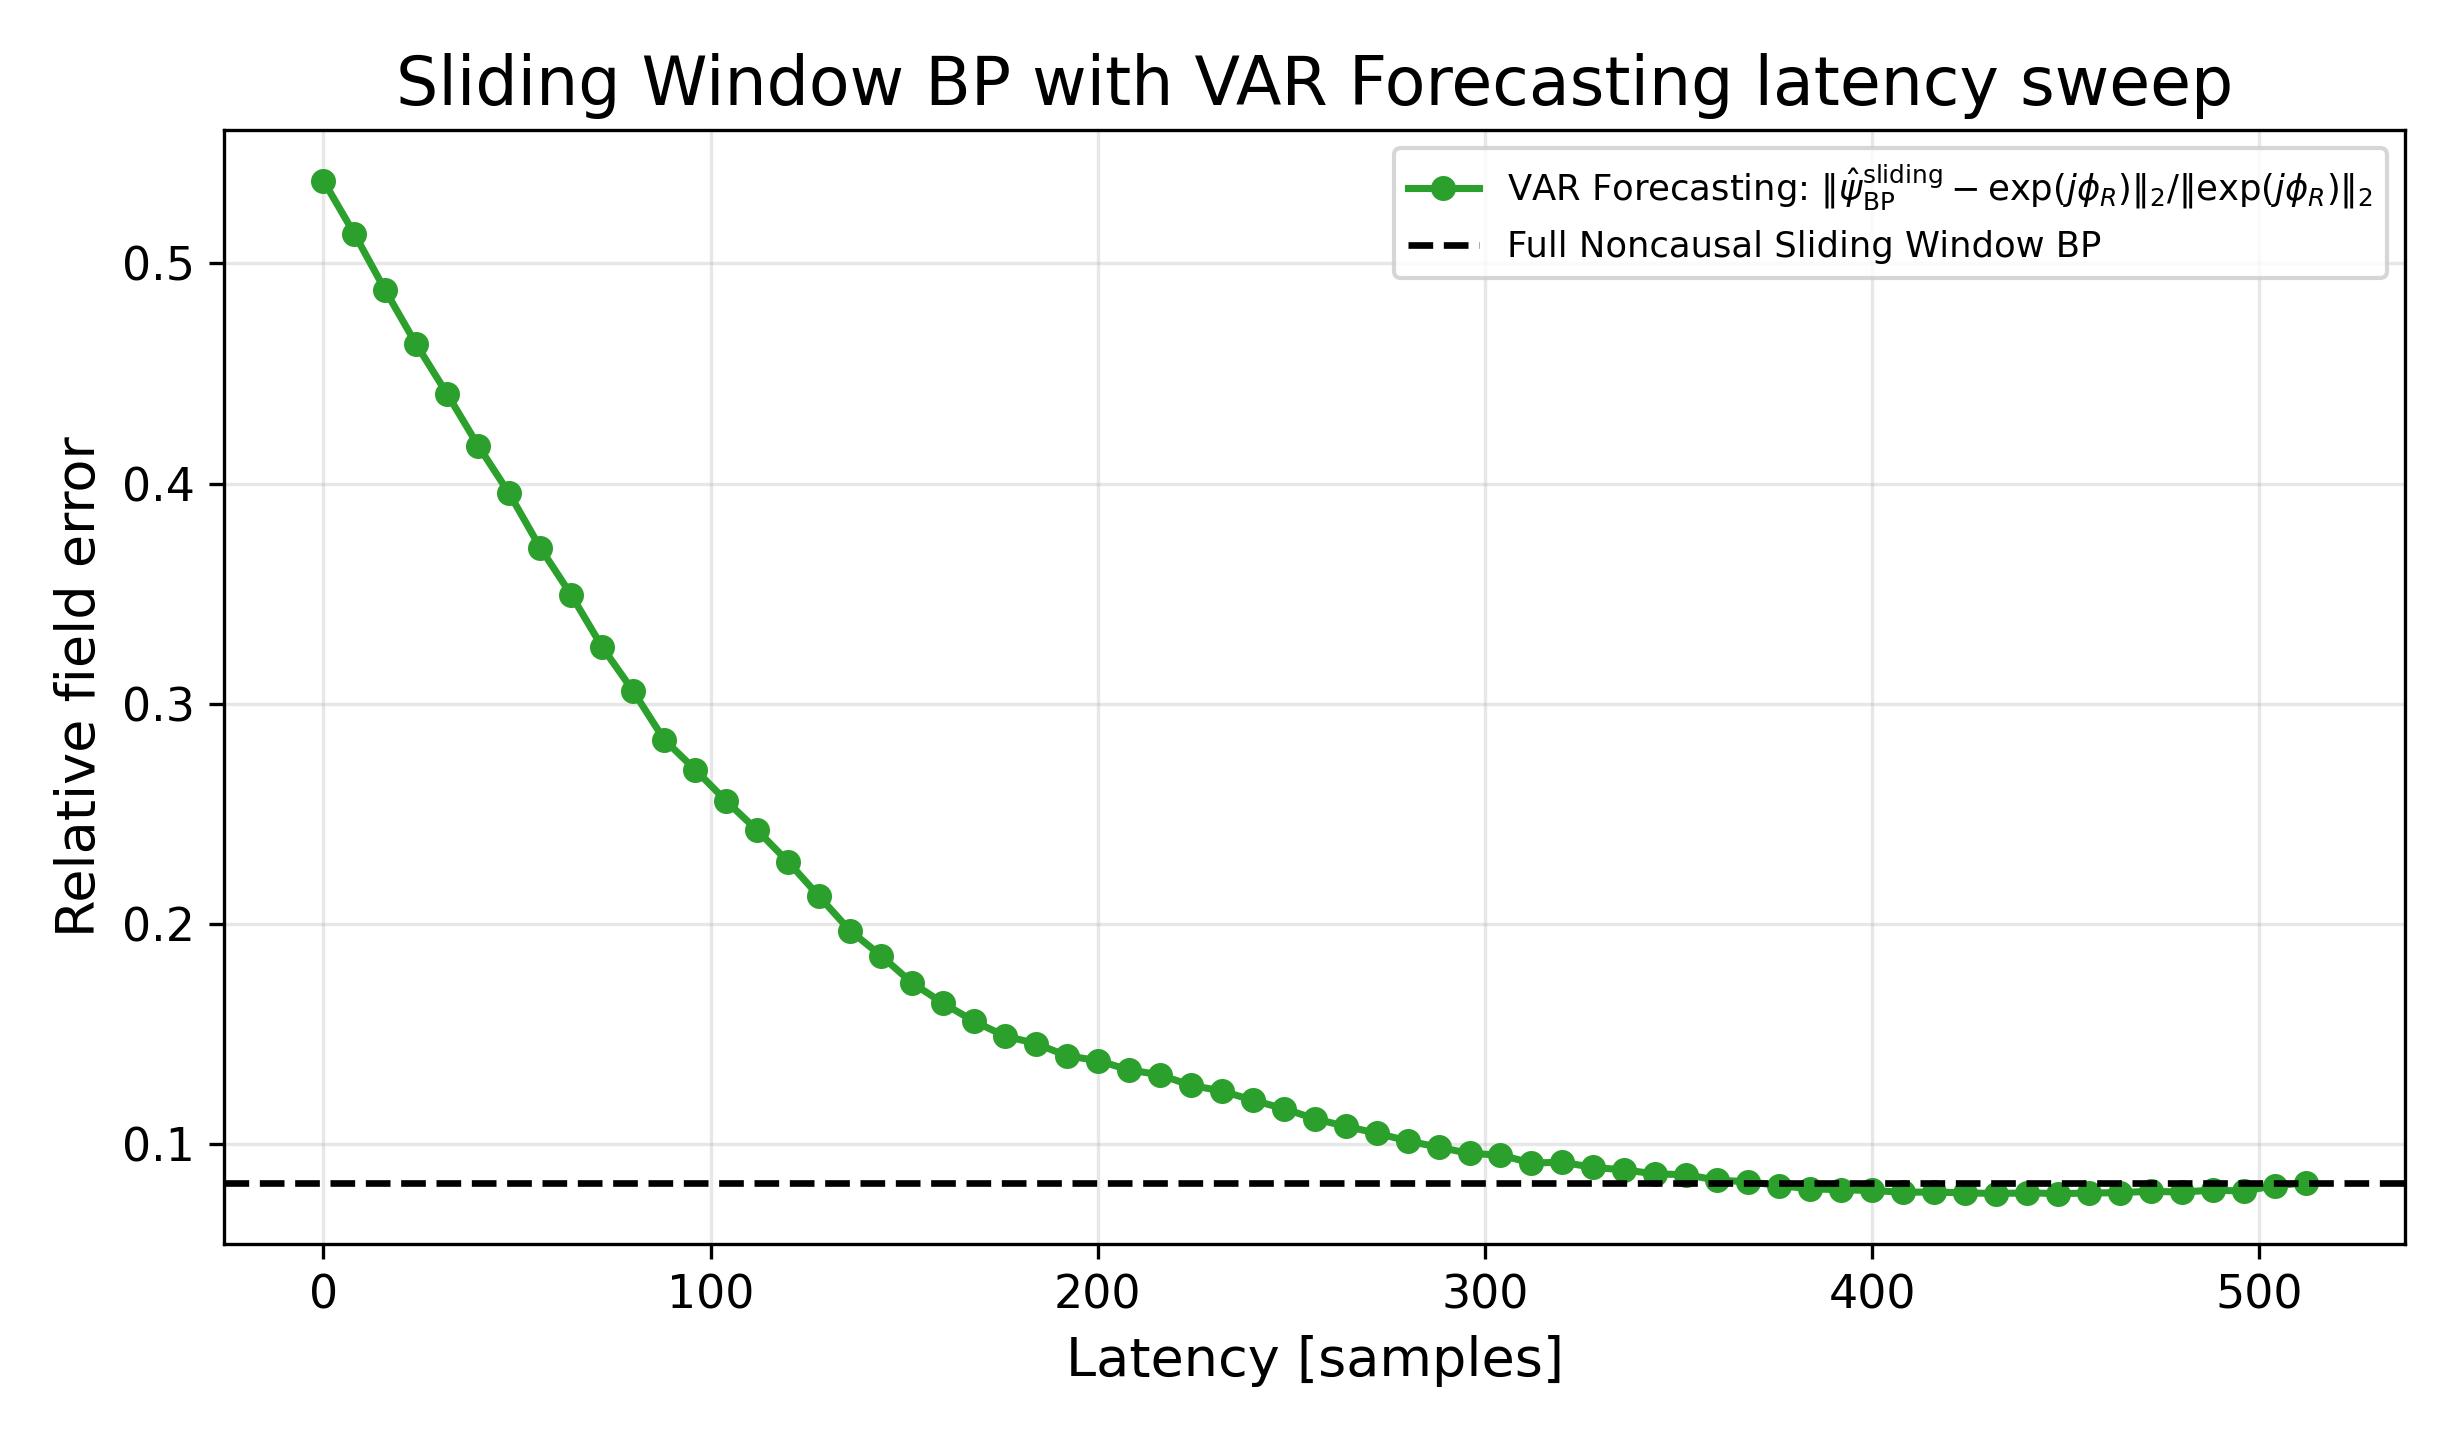
\includegraphics[width=0.85\linewidth]{../figures/sliding_window_bp_latency_error_overlay.png}
    \\\vspace{0.5em}
    \small Figure 3: Relative field error $\frac{\left\| \psi_{\mathrm{BP}}^{\mathrm{sliding}} \left[ k \right] - \exp \left( j \overline{\phi}_{\mathrm{R}} \left[ k \right] \right) \right\|_2}{\left\| \exp \left( j \overline{\phi}_{\mathrm{R}} \left[ k \right] \right) \right\|_2}$ for fixed $M = 1024$ and varying latencies $L$.
\end{frame}

\begin{frame}{Towards Real-Time Backpropagation}
    \centering
    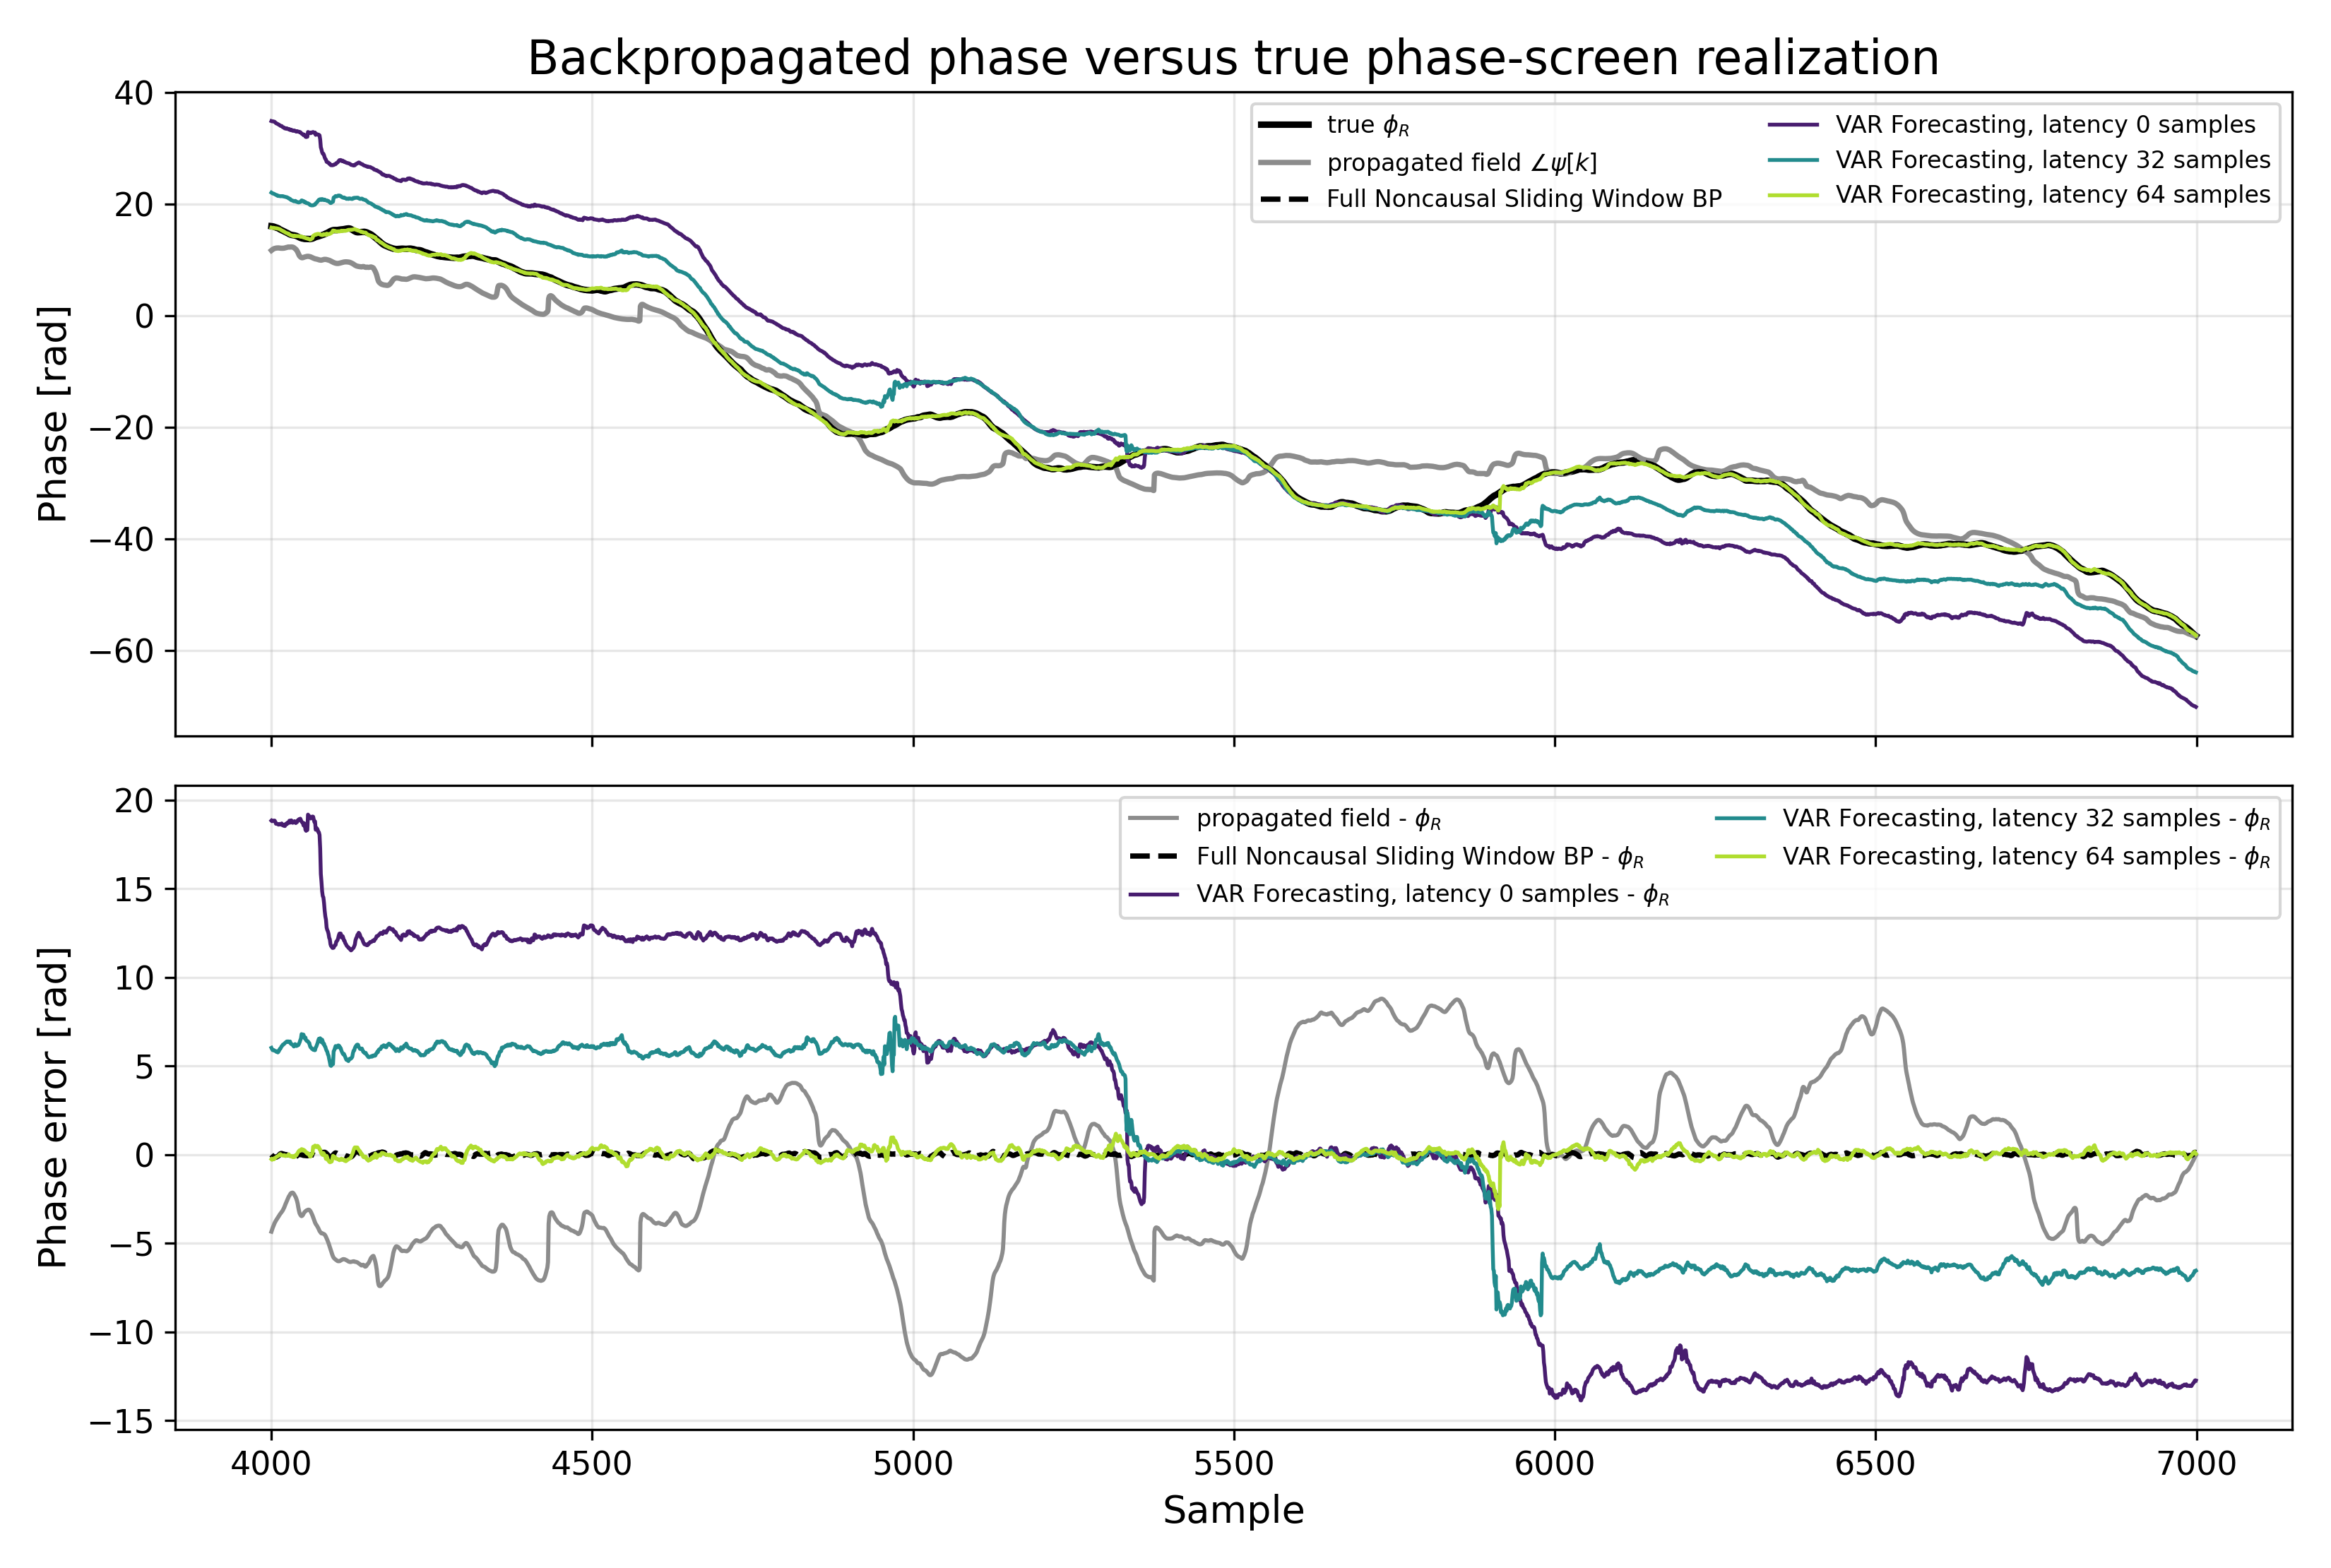
\includegraphics[width=0.9\linewidth]{../figures/phase_sliding_window_bp_var_forecasting_true_phi_R.png}
    \\\vspace{0.5em}
    \small Figure 4: Comparison between the true refractive phase $\overline{\phi}_{\mathrm{R}} \left[ k \right]$ and the estimated phase obtained with the sliding window BP for different latencies.
\end{frame}

\section{Remarks on $\rho_{\mathrm{F}} / v_{\mathrm{eff}}$ Estimation}
\begin{frame}{Remarks on $\rho_{\mathrm{F}} / v_{\mathrm{eff}}$ Estimation}
    \begin{itemize}
        \item In \parencite{breitschMitigationGlobalNavigation2023}, $\rho_{\mathrm{F}} / v_{\mathrm{eff}}$ estimates were obtained by performing an inverse mapping of the scintillation intensity index $S_4$ and the decorrelation time $\tau_0$; (This mapping is not very clear in their work, so it can be difficult to implement this)
        \item On the problem of identifying the position of equatorial plasma bubbles using GNSS radio occultation measurements, \parencite{alfonsoBackPropagationMethod2024} propose to find the phase-screen location by minimizing the standard deviation of the measured scintillation amplitude. Similarly, it should be possible to instead search $\rho_{\mathrm{F}} / v_{\mathrm{eff}}$ using the same approach;
        \item Althogh we investigate the use of machine learning models for identifying $\rho_{\mathrm{F}} / v_{\mathrm{eff}}$, the proposed methods are not suitable for real-time applications.
    \end{itemize}
\end{frame}

\begin{frame}{Remarks on $\rho_{\mathrm{F}} / v_{\mathrm{eff}}$ Estimation}
    Thus, I understand that a reasonable (and easy) way of estimating $\rho_{\mathrm{F}} / v_{\mathrm{eff}}$ in real-time consists in defining a bank of inverse propagation kernels defined with linearly spaced values of $\rho_{\mathrm{F}} / v_{\mathrm{eff}}$, and performing backpropagation of a measured scintillation signal for each of them. The most suitable kernel can be chosen as the one that minimizes the scintillation amplitude standard deviation.
\end{frame}

\section{Short-Term Goals for ION GNSS+ 2026}

\begin{frame}{Short-Term Goals for ION GNSS+ 2026}
    \begin{enumerate}
        \item Use a scintillation signal dataset obtained from tracking loops (I would choose either a standard Kalman filter--Wiener model only or an FLL-Assisted PLL--closer to what is implemented in CoTS receivers)
        \item Implement three machine learning models for forecasting, comparing with the VAR model baseline (LSTM/GRU, PATCHTST--Transformer, NHITS--Neural Hierarchical Interpolation)
        \item Implement the bank of filters for estimating $\rho_{\mathrm{F}} / v_{\mathrm{eff}}$
        \item Evaluate loss-of-lock and cycle-slips mitigation statistics.
        \item It would be great to validate the results using real measurements. Despite the known problems on the signal processing methods implemented on CoTS receivers, I believe that backpropagation may help on the scintillation mitigation and monitoring using .
    \end{enumerate}
\end{frame}

\appendix % frames below this line won't count toward total slide numbering

\begin{frame}[allowframebreaks]{References}
    \printbibliography[heading=none]
\end{frame}

\end{document}
